\documentclass[]{article}
\usepackage[T1]{fontenc}
\usepackage{lmodern}
\usepackage{amssymb,amsmath}
\usepackage{ifxetex,ifluatex}
\usepackage{fixltx2e} % provides \textsubscript
% use upquote if available, for straight quotes in verbatim environments
\IfFileExists{upquote.sty}{\usepackage{upquote}}{}
\ifnum 0\ifxetex 1\fi\ifluatex 1\fi=0 % if pdftex
  \usepackage[utf8]{inputenc}
\else % if luatex or xelatex
  \ifxetex
    \usepackage{mathspec}
    \usepackage{xltxtra,xunicode}
  \else
    \usepackage{fontspec}
  \fi
  \defaultfontfeatures{Mapping=tex-text,Scale=MatchLowercase}
  \newcommand{\euro}{€}
\fi
% use microtype if available
\IfFileExists{microtype.sty}{\usepackage{microtype}}{}
\usepackage[margin=1in]{geometry}
\usepackage{graphicx}
% Redefine \includegraphics so that, unless explicit options are
% given, the image width will not exceed the width of the page.
% Images get their normal width if they fit onto the page, but
% are scaled down if they would overflow the margins.
\makeatletter
\def\ScaleIfNeeded{%
  \ifdim\Gin@nat@width>\linewidth
    \linewidth
  \else
    \Gin@nat@width
  \fi
}
\makeatother
\let\Oldincludegraphics\includegraphics
{%
 \catcode`\@=11\relax%
 \gdef\includegraphics{\@ifnextchar[{\Oldincludegraphics}{\Oldincludegraphics[width=\ScaleIfNeeded]}}%
}%
\ifxetex
  \usepackage[setpagesize=false, % page size defined by xetex
              unicode=false, % unicode breaks when used with xetex
              xetex]{hyperref}
\else
  \usepackage[unicode=true]{hyperref}
\fi
\hypersetup{breaklinks=true,
            bookmarks=true,
            pdfauthor={Brian C., James Q., Rohan F., Sharad G.},
            pdftitle={Sandwich Tycoon},
            colorlinks=true,
            citecolor=blue,
            urlcolor=blue,
            linkcolor=magenta,
            pdfborder={0 0 0}}
\urlstyle{same}  % don't use monospace font for urls
\setlength{\parindent}{0pt}
\setlength{\parskip}{6pt plus 2pt minus 1pt}
\setlength{\emergencystretch}{3em}  % prevent overfull lines
\setcounter{secnumdepth}{0}

\title{Sandwich Tycoon}
\author{Brian C., James Q., Rohan F., Sharad G.}
\date{}

\begin{document}

\begin{center}
\huge Sandwich Tycoon \\[0.2cm]
\end{center}
\begin{center}
\large \emph{Brian C., James Q., Rohan F., Sharad G.}\\[0.1cm]
\end{center}
\normalsize


\subsubsection{Initial Thoughts}\label{initial-thoughts}

After plotting histograms and scatterplots of the historical data, it
was evident that:

\begin{itemize}
\itemsep1pt\parskip0pt\parsep0pt
\item
  Demand fluctuated heavily day to day
\item
  James was often undersupplying all types of sandwiches (i.e.~demand
  \textgreater{} supply)
\item
  There were no imminent customer patterns based on day of sale (e.g
  first day of each week had XX sales) or sandwich conditionality
  (e.g.~if previous day sold X, next day would sell Y)
\item
  No obvious long-term demand trend upwards or downwards (linear
  regression, $a<.02$ and $r2<.0001$ for all types)
\end{itemize}

See Appendix:Initial Graphs

\subsubsection{Objective}\label{objective}

To maximize total sandwich profits over a 130-day period by estimating
probability of demand and producing a fixed or variable quantity of
supply.

\subsubsection{General Strategy}\label{general-strategy}

Sandwiches sold is a discrete variable and therefore can be estimated
using a probability mass function. We forecasted demand using two
different probability distributions, namely:

\begin{enumerate}
\def\labelenumi{\arabic{enumi}.}
\item
  Historical frequency: This distribution would match the probability
  ($X=x$) of the preceding period.
\item
  Poisson distribution: This is an applicable distribution because we
  want the probability of a discrete number of occurences in a fixed
  period of time (i.e.~sandwiches sold in a day)
\end{enumerate}

James previously supplied sandwiches at a mostly fixed amount. We used a
fixed supply model for the historical distribution but modeled the
poisson distribution under both fixed and variable supply assumptions.

A 130-day period was chosen to match the timeline of the given data.
This allows for direct benchmarking (given below assumptions) against 1)
profits that James actually made in the preceding 130 days, and 2) a
gold standard profit margin that was achievable over 130 days if supply
always met demand every day.

\subsubsection{General Assumptions}\label{general-assumptions}

\begin{itemize}
\itemsep1pt\parskip0pt\parsep0pt
\item
  Demand for each sandwich type is independent. What a customer orders
  is independent of what was ordered before.
\item
  Each customer only counts towards demand of one sandwich type.
  Therefore, if a customer wanted ham but it was sold out and turkey was
  bought instead, demand would count as 1 ham, 0 turkey. This means the
  sum of total demand equals the total number of customers who visited
  on a given day
\item
  Future demand will closely match historical demand. Again, there was
  no evident long-term trend and we have no information to assume a
  drastic drop or growth over the next 130 days (e.g.~more people in the
  building, other competition, vegan explosion, swine flu epidemic)
\item
  There are no added fixed costs to increasing supply (e.g.~hiring
  helpers, more preparation space/tools)
\item
  Supply goes to waste if not sold in a day. We vary this assumption in
  our second Poisson distribution model\\
\end{itemize}

\subsubsection{Profit Results}\label{profit-results}

\paragraph{A) Previously achieved -
\$12,828}\label{a-previously-achieved---12828}

Given James' actual supply and demand over the 130-day period, he
achieved the following:

\begin{table}[!htbp]
  \label{} 
\begin{tabular}{@{\extracolsep{5pt}} ccccc} 
\\[-1.8ex]\hline 
\hline \\[-1.8ex] 
type & revenue & cost & profit \\ 
\hline \\[-1.8ex] 
ham & $12,012$ & $7,175$ & $4,837$ \\ 
turkey & $14,066$ & $8,960$ & $5,106$ \\ 
veggie & $5,960$ & $3,075$ & $2,885$ \\ 
total & $32,038$ & $19,210$ & $12,828$ \\ 
\hline \\[-1.8ex] 
\end{tabular} 
\end{table}

\paragraph{B) Historical Probability Distribution -
\$13,858}\label{b-historical-probability-distribution---13858}

We used historical frequency of each demand amount to determine the
probability ($X=x$) of each sandwich sold on a given day. With this
probability distribution, we simulated 10,000 trials over a 130-day
period to get our demand estimate. Under our assumption of fixed supply,
we calculated the revenue, cost, and profit for each fixed number of
sandwiches produced (over the demand range of each sandwich type).

The results demonstrate that the optimal fixed number of sandwiches to
supply per day is equal to the expected value, which under a specific
frequency distribution is the highest frequency value (ham: $n=15$
$p=0.123$, turkey: $n=20$ $p=0.1$, veggie: $n=13$ $p=.138$).

\begin{table}[!htbp]
  \label{} 
\begin{tabular}{@{\extracolsep{5pt}} ccccc} 
\\[-1.8ex]\hline 
\hline \\[-1.8ex] 
type & revenue & cost & profit \\ 
\hline \\[-1.8ex] 
ham & $11,765$ & $6,825$ & $4,940$ \\ 
turkey & $16,003$ & $10,400$ & $5,603$ \\ 
veggie & $7,540$ & $4,225$ & $3,315$ \\ 
total & $35,308$ & $21,450$ & $13,858$ \\ 
\hline \\[-1.8ex] 
\end{tabular} 
\end{table}

\textbf{(insert charts - frequency distribution, marginal profit
curve?)}

\paragraph{C) Poisson Distribution - Fixed
Supply}\label{c-poisson-distribution---fixed-supply}

\textbf{include that lambda = expected value = optimum supply level}

\subparagraph{Without Storage (unsold sandwiches are
wasted)}\label{without-storage-unsold-sandwiches-are-wasted}

\begin{verbatim}
## stat_bin: binwidth defaulted to range/30. Use 'binwidth = x' to adjust this.
## stat_bin: binwidth defaulted to range/30. Use 'binwidth = x' to adjust this.
## stat_bin: binwidth defaulted to range/30. Use 'binwidth = x' to adjust this.
\end{verbatim}

\begin{verbatim}
## Warning: position_stack requires constant width: output may be incorrect
## Warning: position_stack requires constant width: output may be incorrect
## Warning: position_stack requires constant width: output may be incorrect
\end{verbatim}

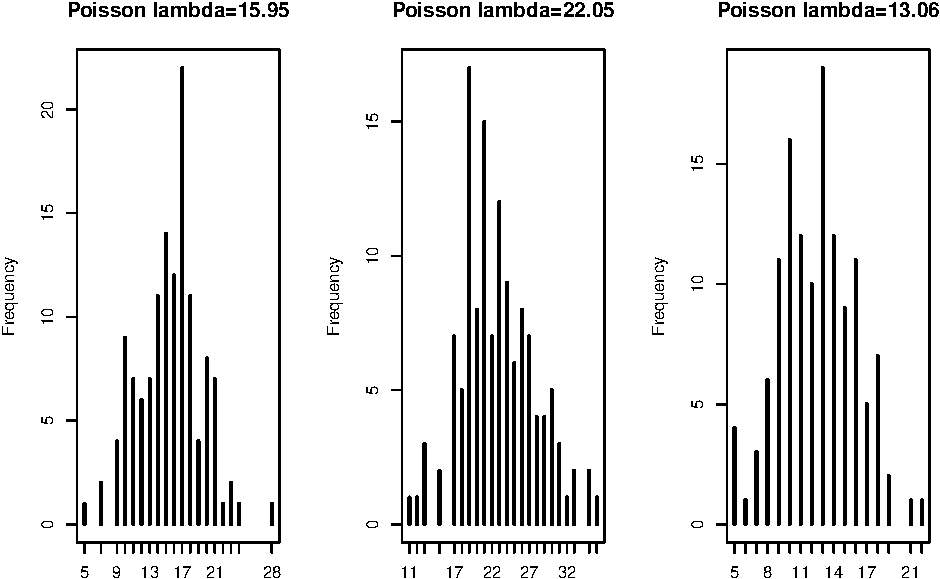
\includegraphics{./IS606_Sandwich_files/figure-latex/unnamed-chunk-2.pdf}

\subparagraph{With Storage (unsold sandwiches are put back into
supply)}\label{with-storage-unsold-sandwiches-are-put-back-into-supply}

\paragraph{D) Poisson Distribution - Variable
Supply}\label{d-poisson-distribution---variable-supply}

\paragraph{E) Gold Standard - \$17,631}\label{e-gold-standard---17631}

This is the profit that would have been made if supply=demand each day
so that no sandwich was wasted and every customer was satisfied.
Comparing the previous methods as percent of gold standard achieved, we
see the poisson variable supply model yielded XX\% while the poisson
fixed model and historical probability model yielded XX\% and $78.6\%$,
respectively.

\subsubsection{Recommendations}\label{recommendations}

\begin{itemize}
\itemsep1pt\parskip0pt\parsep0pt
\item
  If fixed supply, produce at rate of expected value
\item
  Poisson distribution fit historical data very well - can use as
  distribution function going forward
\item
  Consider investing in fridge, etc. to prolong product shelf life
\item
  Being able to carry over supply day-to-day greatly increase expected
  profit
\end{itemize}

\subsubsection{Limitations}\label{limitations}

\begin{itemize}
\itemsep1pt\parskip0pt\parsep0pt
\item
  Simple model assuming external factors not changing
\item
  Will historical demand \textasciitilde{} Future demand?
\item
  Covariance. If no turkey is produced, could some/all switch to higher
  margin ham?
\item
  Fixed supply costs in real world would likely increase
\item
  In variable model, 3-day old sandwich is as `desirable' as fresh one
\end{itemize}

\section{Appendix}\label{appendix}

\subsubsection{Initial Graphs}\label{initial-graphs}

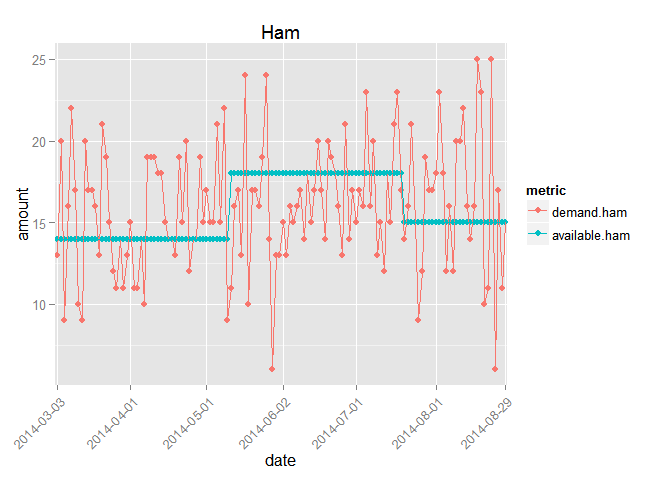
\includegraphics{./IS606_Sandwich_files/figure-latex/unnamed-chunk-41.pdf}
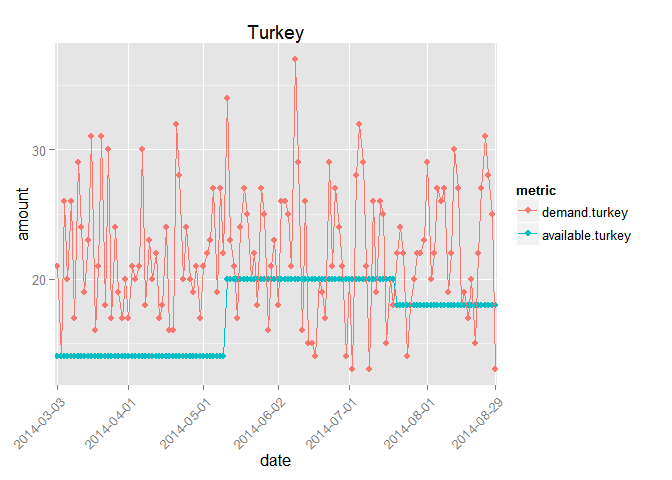
\includegraphics{./IS606_Sandwich_files/figure-latex/unnamed-chunk-42.pdf}
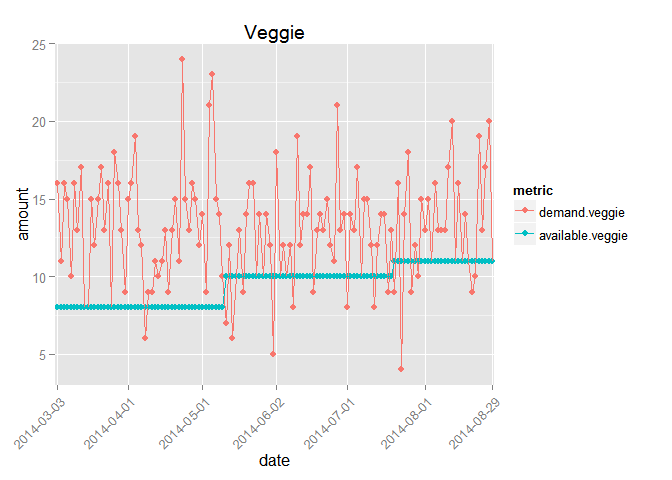
\includegraphics{./IS606_Sandwich_files/figure-latex/unnamed-chunk-43.pdf}

\end{document}
